\Opensolutionfile{ans}[ans/ansTN-CaoThang246]

\noindent \textbf{PHẦN I. Câu trắc nghiệm có nhiều phương án lựa chọn (6đ). Thí sinh trả lời từ câu 1 đến câu 18. Mỗi câu hỏi thí sinh chỉ chọn một phương án}
\vspace{0.2cm}

\begin{ex}	\macau{ID: VL12-CT246-C01}Khi nói về thang đo nhiệt độ Kelvin và Celsius, kết luận nào sau đây là sai?
	\choice
	{Nhiệt độ trong thang đo Kelvin được ký hiệu là $T$, có đơn vị K}
	{\True Một độ chia trên thang nhiệt độ Kelvin có giá trị gấp 273 lần một độ chia trên thang nhiệt độ Celsius}
	{Mối liên hệ về các giá trị nhiệt độ giữa hai thang đo là: $T(\text{K})=t(^\circ\text{C})+273,15$}
	{Nhiệt độ trong thang nhiệt độ Celsius được ký hiệu là $t$, có đơn vị $^\circ\text{C}$}
	loigiai{
		Độ chia trong thang nhiệt độ Kelvin và thang nhiệt độ Celsius có độ rộng bằng nhau ($1\text{ K} = 1^\circ\text{C}$). Do đó, phát biểu khẳng định độ chia này gấp 273 lần độ chia kia là hoàn toàn sai}
\end{ex}

\begin{ex}	\macau{ID: VL12-CT246-C02}Trong thang nhiệt độ Celsius, phát biểu nào sau đây là sai?
	\choice
	{Kí hiệu nhiệt độ là $t(^\circ\text{C})$}
	{Những nhiệt độ thấp hơn $0^\circ\text{C}$ gọi là nhiệt độ âm}
	{\True Nhiệt độ của nước đá đang tan lớn hơn $0^\circ\text{C}$}
	{Nhiệt độ sôi của nước lớn hơn $0^\circ\text{C}$}
	\loigiai{
		Trong nhiệt giai Celsius, nhiệt độ của nước đá đang tan dưới áp suất tiêu chuẩn được chọn làm vạch mốc cố định bằng đúng $0^\circ\text{C}$, không phải lớn hơn $0^\circ\text{C}$}
\end{ex}

\begin{ex}	\macau{ID: VL12-CT246-C03}Trong công thức tính nhiệt lượng chuyển pha nóng chảy $Q = \lambda \cdot m$, đại lượng $\lambda$ được gọi là
	\choice
	{nhiệt hóa hơi riêng}
	{nhiệt nóng chảy toàn phần}
	{nhiệt lượng cần cung cấp cho chất rắn trong quá trình nóng chảy}
	{\True nhiệt nóng chảy riêng của chất rắn}
	\loigiai{
		Trong hệ thức tính nhiệt lượng nóng chảy, đại lượng $\lambda$ đại diện cho nhiệt nóng chảy riêng của chất rắn kết tinh, đặc trưng cho bản chất liên kết cấu trúc của chất đó}
\end{ex}

\begin{ex}	\macau{ID: VL12-CT246-C04}Phát biểu nào sau đây là sai về nhiệt nóng chảy riêng của chất rắn? Nhiệt nóng chảy riêng của chất rắn:
	\choice
	{là nhiệt lượng cần cung cấp để làm nóng chảy hoàn toàn $1\text{ kg}$ chất đó ở nhiệt độ nóng chảy}
	{có đơn vị tiêu chuẩn trong hệ SI là $\text{J/kg}$}
	{phụ thuộc chặt chẽ vào bản chất cấu trúc của chất rắn}
	{\True là nhiệt lượng cần cung cấp để làm nóng chảy hoàn toàn khối lượng lượng chất đó ở nhiệt độ nóng chảy}
	\loigiai{
		Nhiệt nóng chảy riêng $\lambda$ theo định nghĩa chỉ tính cho một đơn vị khối lượng tiêu chuẩn ($1\text{ kg}$) vật chất ở nhiệt độ nóng chảy, phát biểu D nói cho toàn bộ "lượng chất đó" (tương ứng với nhiệt nóng chảy $Q$) là sai}
\end{ex}

\begin{ex}	\macau{ID: VL12-CT246-C05}Phát biểu nào sau đây là sai khi nói về hiện tượng nóng chảy và sự đông đặc?
	\choice
	{Đối với một chất rắn kết tinh nhất định, nếu nóng chảy ở nhiệt độ nào thì sẽ đông đặc ở nhiệt độ ấy}
	{Các chất khác nhau sẽ nóng chảy (hay đông đặc) ở nhiệt độ hoàn toàn khác nhau}
	{\True Nhiệt độ của vật sẽ tăng dần trong quá trình nóng chảy và giảm dần trong quá trình đông đặc}
	{Phần lớn các chất nóng chảy (hay đông đặc) ở một nhiệt độ cố định xác định}
	\loigiai{
		Trong suốt tiến trình chuyển pha (nóng chảy hoặc đông đặc), dù hệ tiếp tục trao đổi nhiệt lượng với môi trường nhưng năng lượng này chỉ phục vụ thay đổi liên kết phân tử, do đó nhiệt độ của vật luôn giữ cố định không đổi. Nhận định C sai}
\end{ex}

\begin{ex}	\macau{ID: VL12-CT246-C06}Trong quá trình chất khí nhận nhiệt lượng $Q$ và thực hiện sinh công $A$, nội năng của một lượng khí biến thiên một lượng tuân theo biểu thức $\Delta U = A + Q$. Khi đó, các dấu đại số của $A$ và $Q$ phải thỏa mãn điều kiện nào dưới đây?
	\choice
	{$Q>0$ và $A>0$}
	{ $Q<0$ và $A>0$}
	{$Q<0$ và $A<0$}
	{\True $Q>0$ và $A<0$}
	\loigiai{
		Theo quy ước dấu của Nguyên lí I nhiệt động lực học:
		- Hệ chất khí nhận nhiệt lượng từ môi trường ngoài $\Rightarrow Q > 0$.
		- Hệ chất khí sinh công (thực hiện công) tác dụng lên ngoại cảnh $\Rightarrow A < 0$}
\end{ex}

\begin{ex}	\macau{ID: VL12-CT246-C07}Câu nào sau đây phát biểu về đặc trưng chuyển động của các phân tử là không đúng?
	\choice
	{Các phân tử chuyển động hỗn loạn càng nhanh thì nhiệt độ của vật càng cao}
	{Các phân tử chất khí chuyển động hoàn toàn hỗn độn và không dao động quanh một vị trí cố định}
	{\True Chuyển động nhiệt hỗn loạn của các phân tử là do lực tương tác phân tử trực tiếp gây ra}
	{Các phân tử cấu tạo nên vật chất luôn chuyển động hỗn loạn không ngừng}
	\loigiai{
		Chuyển động của các phân tử là chuyển động nhiệt tự thân, luôn diễn ra không ngừng độc lập với lực tương tác. Lực tương tác phân tử chỉ đóng vai trò quy định cấu trúc khoảng cách xa gần và giới hạn không gian chuyển động của các thể}
\end{ex}

\begin{ex}	\macau{ID: VL12-CT246-C08}Nếu hai vật có nhiệt độ ban đầu khác nhau được đặt tiếp xúc nhiệt với nhau, quá trình truyền nhiệt tự phát giữa chúng sẽ dừng lại khi
	\choice
	{một trong hai vật đạt tới vạch mức nhiệt độ $0^\circ\text{C}$}
	{nội năng bên trong của hai vật đạt trạng thái bằng nhau}
	{\True nhiệt độ của hai vật biến đổi đạt ngưỡng bằng nhau}
	{nhiệt dung riêng của hai vật bằng nhau}
	\loigiai{
		Sự chênh lệch nhiệt độ là nguyên nhân duy nhất thúc đẩy dòng truyền nhiệt tự phát từ vật nóng sang vật lạnh. Quá trình truyền nhiệt sẽ chấm dứt khi hệ thiết lập trạng thái cân bằng nhiệt, tức là nhiệt độ của hai vật bằng nhau}
\end{ex}

\begin{ex}	\macau{ID: VL12-CT246-C09}Thông thường, một nhiệt kế rượu tiêu chuẩn có giới hạn đo an toàn từ $-115^\circ\text{C}$ đến $78,5^\circ\text{C}$. Không thể sử dụng chiếc nhiệt kế này để đo đạc chỉ số nhiệt độ nào dưới đây?
	\choice
	{\True Nhiệt độ sôi của nước tinh khiết ở áp suất tiêu chuẩn}
	{Nhiệt độ của khí quyển vùng băng giá}
	{Nhiệt độ cơ thể của con người}
	{Nhiệt độ của khối nước đá đang tan}
	\loigiai{
		Nhiệt độ sôi của nước tinh khiết ở áp suất tiêu chuẩn bằng $100^\circ\text{C}$. Trị số này vượt quá giới hạn đo tối đa của nhiệt kế rượu ($78,5^\circ\text{C}$, vạch mức rượu sẽ bị sôi và phá hủy nhiệt kế), nên không thể đo được}
\end{ex}

\begin{ex}	\macau{ID: VL12-CT246-C10}Cho hằng số nhiệt dung riêng của nước là $4180\text{ J/(kg.K)}$ và ẩn nhiệt hóa hơi riêng của nước bằng $2,3 \cdot 10^6\text{ J/kg}$. Tổng nhiệt lượng cần cung cấp để làm cho $10\text{ kg}$ nước lỏng đang ở vạch nhiệt độ $25^\circ\text{C}$ hóa hơi hoàn toàn là
	\choice
	{$26135\text{ J}$}
	{$24045\text{ J}$}
	{\True $26135\text{ kJ}$}
	{$24045\text{ kJ}$}
	\loigiai{
		Tiến trình thu nhiệt gồm hai giai đoạn liên tiếp:
		- Giai đoạn 1: Thu nhiệt để nâng nhiệt độ của khối nước từ $25^\circ\text{C} \rightarrow 100^\circ\text{C}$:
		$$Q_1 = m \cdot c \cdot (t_{\text{sôi}} - t_0) = 10 \cdot 4180 \cdot (100 - 25) = 3135000\text{ J}$$
		- Giai đoạn 2: Thu ẩn nhiệt để hóa hơi hoàn toàn lượng nước sôi ở $100^\circ\text{C}$:
		$$Q_2 = m \cdot L = 10 \cdot 2,3 \cdot 10^6 = 23000000\text{ J}$$
		Tổng nhiệt lượng toàn phần cần thiết phải cung cấp:
		$$Q = Q_1 + Q_2 = 3135000 + 23000000 = 26135000\text{ J} = 26135\text{ kJ}$$}
\end{ex}

\begin{ex}	\macau{ID: VL12-CT246-C11}Khi nhiệt độ nội tại của một hệ vật chất bị dâng tăng lên thì
	\choice
	{nội năng tổng hợp của vật bị giảm sụt}
	{động năng chuyển động nhiệt trung bình của các phân tử cấu tạo nên vật giảm}
	{nội năng của vật giữ hằng số không thay đổi}
	{\True động năng chuyển động nhiệt trung bình của các phân tử cấu tạo nên vật tăng}
	\loigiai{
		Nhiệt độ là đại lượng thước đo vĩ mô đặc trưng cho động năng chuyển động nhiệt trung bình của các phân tử cấu tạo nên vật. Khi nhiệt độ tăng, các phân tử chuyển động hỗn loạn càng nhanh, đồng nghĩa động năng trung bình của chúng gia tăng}
\end{ex}

\begin{ex}	\macau{ID: VL12-CT246-C12}Câu nào sau đây phát biểu định tính về các lực tương tác phân tử là không đúng?
	\choice
	{\True Lực hút phân tử tuyệt đối không bao giờ có thể lớn hơn lực đẩy phân tử}
	{Lực hút phân tử có thể cân bằng bằng với lực đẩy phân tử}
	{Lực tương tác phân tử chỉ đóng vai trò đáng kể khi khoảng cách giữa các phân tử ở rất gần nhau}
	{Lực hút phân tử có thể lớn hơn lực đẩy phân tử tùy thuộc khoảng cách}
	\loigiai{
		Giữa các phân tử luôn tồn tại đồng thời cả lực hút và lực đẩy phân tử. Khi khoảng cách giữa các phân tử lớn hơn khoảng cách cân bằng $r > r_0$, lực đẩy giảm nhanh hơn lực hút, khiến lực hút chiếm ưu thế và lớn hơn lực đẩy. Nhận định A khẳng định "không thể lớn hơn" là sai}
\end{ex}

\begin{ex}	\macau{ID: VL12-CT246-C13}Người ta thực hiện một công cơ học có độ lớn bằng $360\text{ J}$ nén ép lên một khối khí lí tưởng chứa trong bình, đồng thời truyền cấp thêm cho khối khí một nhiệt lượng bằng $100\text{ J}$. Độ biến thiên nội năng của khí là
	\choice
	{$260\text{ J}$ và nội năng giảm}
	{\True $460\text{ J}$ và nội năng tăng}
	{$500\text{ J}$ và nội năng giảm}
	{$500\text{ J}$ và nội năng tăng}
	\loigiai{
		Theo quy ước dấu Nguyên lí I của nhiệt động lực học:
		- Thực hiện công lên khối khí $\Rightarrow$ Khí nhận công $\Rightarrow A = +360\text{ J}$.
		- Truyền cho khối khí nhiệt lượng $\Rightarrow$ Khí nhận nhiệt $\Rightarrow Q = +100\text{ J}$.
		Độ biến thiên nội năng tổng hợp của hệ khí:
		$$\Delta U = Q + A = 100 + 360 = +460\text{ J}$$
		Vì $\Delta U > 0$ nên nội năng của khối khí gia tăng thêm một lượng bằng $460\text{ J}$}
\end{ex}

\begin{ex}	\macau{ID: VL12-CT246-C14}Hai chiếc cốc thủy tinh giống hệt nhau chứa nước nóng dóng chung một thềm môi trường xung quanh có suất tỏa nhiệt như nhau. Theo dõi chuyển động nhiệt thấy nước ở cốc thứ nhất nguội đi một lượng $15^\circ\text{C}$ trong vòng $5\text{ phút}$, trong khi nước ở cốc thứ hai chỉ nguội đi một lượng $10^\circ\text{C}$ cũng trong vòng $5\text{ phút}$. Nguyên nhân của hiện tượng này là do
	\choice
	{lượng lượng nước chứa bên trong cốc thứ hai ít hơn so với cốc một}
	{nước chứa trong cốc thứ hai có vạch nhiệt độ ban đầu cao hơn cốc thứ nhất}
	{lượng lượng nước chứa bên trong cốc thứ hai nhiều hơn so với cốc một}
	{\True nước chứa trong cốc thứ hai có vạch nhiệt độ ban đầu thấp hơn cốc thứ nhất}
	\loigiai{
		Tốc độ truyền nhiệt, tỏa nhiệt ra môi trường của một vật phụ thuộc tỉ lệ thuận với độ chênh lệch nhiệt độ giữa vật và môi trường xung quanh (định luật làm lạnh Newton). Cốc thứ hai nguội đi chậm hơn (chỉ giảm $10^\circ\text{C}$ so với $15^\circ\text{C}$ của cốc một trong cùng thời gian) chứng tỏ hiệu nhiệt độ giữa nó và môi trường nhỏ hơn, tức là nhiệt độ ban đầu của cốc thứ hai thấp hơn cốc thứ nhất}
\end{ex}

\begin{ex}	\macau{ID: VL12-CT246-C15}Nhiệt lượng $Q$ cần thiết cung cấp để làm gia tăng nhiệt độ của một khối lượng chất m có nhiệt dung riêng $c\text{ (J/kg.K)}$ từ thềm nhiệt độ ban đầu $t_1$ đạt dâng lên tới vạch nhiệt độ $t_2$ tuân theo công thức là
	\choice
	{\True $Q=mc(t_2-t_1)$}
	{$Q=mc(t_2 \cdot t_1)$}
	{$Q=mc(t_2/t_1)$}
	{$Q=mc(t_2+t_1)$}
	\loigiai{
		Công thức định lượng tính nhiệt lượng thu vào để làm thay đổi nhiệt độ của một hệ vật chất từ trạng thái $t_1 \rightarrow t_2$ là: $Q = m \cdot c \cdot (t_2 - t_1) = m \cdot c \cdot \Delta t$}
\end{ex}

\begin{ex}	\macau{ID: VL12-CT246-C16}Ba quả cầu có khối lượng cơ học hoàn toàn bằng nhau, được làm bằng các chất nhôm, sắt và đồng. Biết hằng số nhiệt dung riêng của nhôm là $880\text{ J/(kg.K)}$, của sắt bằng $460\text{ J/(kg.K)}$, và của đồng bằng $380\text{ J/(kg.K)}$. Quả cầu bằng chất nào sẽ có độ tăng nhiệt độ nhiều nhất nếu ta cấp cho chúng cùng một lượng nhiệt lượng như nhau?
	\choice
	{Quả cầu bằng Sắt}
	{\True Quả cầu bằng Đồng}
	{Quả cầu bằng Nhôm}
	{Cả hai quả cầu Sắt và Đồng tăng như nhau}
	\loigiai{
		Từ hệ thức tính nhiệt lượng: $Q = m \cdot c \cdot \Delta t \Rightarrow \Delta t = \frac{Q}{m \cdot c}$. \\
		Vì các quả cầu có cùng khối lượng $m$ và nhận cùng nhiệt lượng $Q$, nên độ gia tăng nhiệt độ $\Delta t$ sẽ tỉ lệ nghịch với hằng số nhiệt dung riêng $c$ của chất liệu. Do quả cầu đồng có hằng số nhiệt dung riêng nhỏ nhất ($c_{\text{đồng}} = 380\text{ J/(kg.K)}$) nên nó sẽ có mức độ tăng nhiệt độ cao nhất}
\end{ex}

\Closesolutionfile{ans}

%%%%%%%%%%%%%%%%%%%%%%%%%%%%%%%%%%%%%%%%%%%%%%%%%%%%%%%%%%%%%%%%%%%%%%%%%
% PHẦN II: CÂU TRẮC NGHIỆM ĐÚNG SAI
%%%%%%%%%%%%%%%%%%%%%%%%%%%%%%%%%%%%%%%%%%%%%%%%%%%%%%%%%%%%%%%%%%%%%%%%%
\noindent \textbf{PHẦN II. Câu trắc nghiệm đúng sai (2đ). Thí sinh trả lời từ câu 1 đến câu 2. Trong mỗi ý a), b), c), d) ở mỗi câu, thí sinh chọn đúng hoặc sai}
\Opensolutionfile{ans}[ans/ansTF-CaoThang246]

\begin{ex}	\macau{ID: VL12-CT246-C17}Cung cấp một lượng nhiệt lượng bằng $1,5\text{ J}$ cho một khối khí lí tưởng chứa bên trong một bình xi-lanh đặt nằm ngang. Khối chất khí giãn nở sinh lực đẩy tấm pít-tông dời chỗ đi được một khoảng hành trình dài $5\text{ cm}$. Biết lực ma sát xuất hiện cản trở chuyển động ở bề mặt tiếp xúc giữa pít-tông và thành vách xi-lanh có độ lớn hằng số bằng $20\text{ N}$ và diện tích mặt tiết diện ngang của pít-tông cho bằng $1\text{ cm}^2$. Xem như pít-tông chuyển động thẳng đều và áp suất khí giữ cố định không đổi trong quá trình giãn nở.
	\choiceTF[t]
	{Độ lớn công cơ học do khối chất khí thực hiện sinh ra giải phóng đạt trị số bằng $1,2\text{ J}$}
	{\True Trị số độ biến thiên nội năng $\Delta U$ đại số của khối khí khí nhận giá trị bằng $+0,5\text{ J}$}
	{\True Trong suốt tiến trình giãn nở cân bằng động học, áp suất tĩnh của chất khí duy trì ở mức bằng $2 \cdot 10^5\text{ Pa}$}
	{Thể tích không gian hình trụ bên trong lòng xi-lanh đã được mở rộng gia tăng thêm một lượng bằng đúng $5\text{ lít}$}
	\loigiai{
		\begin{itemchoice}
			\itemch Quy đổi khoảng hành trình dịch chuyển: $s = 5\text{ cm} = 0,05\text{ m}$. Vì pít-tông chuyển động tịnh tiến thẳng đều, lực đẩy do áp suất khí tác dụng cân bằng động với độ lớn lực ma sát trượt: $F_{\text{đẩy}} = F_{\text{ms}} = 20\text{ N}$. \\
			Độ lớn công cơ học do khối khí sinh ra thực hiện bằng: $A' = F_{\text{đẩy}} \cdot s = 20 \cdot 0,05 = 1,0\text{ J}$.
			\itemch Khí nhận nhiệt lượng $\Rightarrow Q = +1,5\text{ J}$. Khí sinh công đẩy pít-tông $\Rightarrow$ công đại số hệ nhận vào là $A = -A' = -1,0\text{ J}$. Độ biến thiên nội năng tính theo định luật: $\Delta U = Q + A = 1,5 + (-1,0) = +0,5\text{ J}$.
			\itemch Quy đổi diện tích mặt tiết diện pít-tông: $S = 1\text{ cm}^2 = 1 \cdot 10^{-4}\text{ m}^2$. \\
			Áp suất tĩnh nội tại của khối khí tạo lực đẩy pít-tông thỏa mãn hệ thức:
			$$p = \frac{F_{\text{đẩy}}}{S} = \frac{20\text{ N}}{1 \cdot 10^{-4}\text{ m}^2} = 2 \cdot 10^5\text{ Pa}$$
			\itemch Lượng thể tích xi-lanh tăng thêm do pít-tông dời chỗ dịch chuyển bằng:
			$$\Delta V = S \cdot s = 1\text{ cm}^2 \cdot 5\text{ cm} = 5\text{ cm}^3 = 5 \cdot 10^{-6}\text{ m}^3 = 0,005\text{ lít} \text{ (không phải 5 lít)}$$
		\end{itemchoice}
	}
\end{ex}

\begin{ex}	\macau{ID: VL12-CT246-C18}
\immini{
Một học sinh tiến hành thực hiện đun nóng một khối lượng mẫu nước đá ban đầu từ vạch mốc nhiệt độ nóng chảy $0^\circ\text{C}$ cho đến khi khối đá tan chảy hết hoàn toàn thành nước lỏng rồi tiếp tục nâng nhiệt cho đến khi hóa hơi bão hòa trọn vẹn ở vạch điểm sôi $100^\circ\text{C}$. Đồ thị hình vẽ bên biểu diễn mối quan hệ của giá trị lượng nhiệt lượng $Q\text{ (kJ)}$ mà hệ mẫu chất hấp thụ phụ thuộc dóng theo sự thay đổi nhiệt độ $t(^\circ\text{C})$ của nó. Biết các hằng số kĩ thuật chuyển pha: nhiệt nóng chảy riêng của nước đá bằng $3{,}3 \cdot 10^5\text{ J/kg}$, hằng số nhiệt dung riêng nước lỏng bằng $4200\text{ J/(kg.K)}$ và ẩn nhiệt hóa hơi riêng của nước bằng $2{,}3 \cdot 10^6\text{ J/kg}$}{
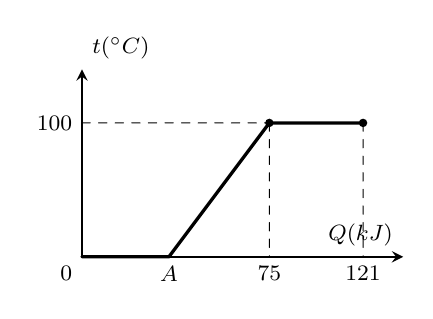
\begin{tikzpicture}[>=stealth, font=\footnotesize, scale=0.85, line cap=round, line join=round]
  \draw[->, thick] (0,0) -- (4.8,0) node[above left] {$Q(\text{kJ})$};
  \draw[->, thick] (0,0) -- (0,2.8) node[above right] {$t(^\circ\text{C})$};
  \node[below left] at (0,0) {$0$};
  
  \coordinate (O) at (0,0);
  \coordinate (A) at (1.3,0);
  \coordinate (B) at (2.8,2.0);
  \coordinate (C) at (4.2,2.0);
  
  \draw[very thick] (O) -- (A) -- (B) -- (C);
  \fill (B) circle (1.8pt);
  \fill (C) circle (1.8pt);
  
  \draw[dashed, thin] (0,2.0) node[left] {$100$} -- (C);
  \draw[dashed, thin] (B) -- (2.8,0) node[below] {$75$};
  \draw[dashed, thin] (C) -- (4.2,0) node[below] {$121$};
  \node[below] at (A) {$A$};
\end{tikzpicture}
}
	\choiceTF[t]
	{Trong phân đoạn đồ thị kí hiệu từ điểm gốc O đến điểm nút A, khối nước đá thu nhận nhiệt lượng từ nguồn ngoài để thực hiện tiến trình tăng nhiệt độ}
	{\True Ngay tại vị trí điểm nút A hiển thị trên trục hoành đồ thị, toàn bộ khối lượng mẫu nước đá đã hoàn toàn chuyển trạng thái sang thể lỏng}
	{Dựa trên thông số trục năng lượng, khối lượng mẫu nước đá học sinh đem làm thí nghiệm có giá trị khối lượng bằng $60\text{ g}$}
	{Nếu học sinh tiếp tục cấp dòng đun cho đến khi toàn bộ lượng nước lỏng hóa hơi hoàn toàn biến mất khỏi bình thì tổng nhiệt lượng cần thiết phải cung cấp bằng đúng $305\text{ kJ}$}
	\loigiai{
		\begin{itemchoice}
			\itemch Đoạn OA nằm ngang ở thềm mức nhiệt độ không đổi $0^\circ\text{C}$, chứng tỏ chất đang hấp thụ nhiệt lượng để phục vụ riêng cho tiến trình chuyển pha nóng chảy tan rã cấu trúc đá, không phải tăng nhiệt độ.
			\itemch Điểm A là điểm mốc kết thúc của đoạn thẳng nằm ngang nóng chảy, cho biết toàn bộ lượng nước đá đã chuyển pha hoàn toàn sang trạng thái thể lỏng ở $0^\circ\text{C}$.
			\itemch Từ đồ thị dóng mốc, lượng nhiệt lượng tiêu hao riêng cho chặng OA nóng chảy đạt mức $Q_{\text{nc}} = 75\text{ kJ} = 75000\text{ J}$. \\
			Khối lượng mẫu nước đá đem dùng làm thí nghiệm được tính toán định lượng bằng:
			$$m = \frac{Q_{\text{nc}}}{\lambda} = \frac{75000\text{ J}}{3{,}3 \cdot 10^5\text{ J/kg}} \approx 0,2273\text{ kg} \approx 227,3\text{ g} \text{ (không phải 60 g)}$$
			\itemch Đoạn nâng nhiệt từ $0^\circ\text{C} \rightarrow 100^\circ\text{C}$ tiêu hao lượng nhiệt $Q_{\text{nâng}} = m \cdot c \cdot \Delta t = 0,2273 \cdot 4200 \cdot 100 \approx 95466\text{ J} \approx 95,5\text{ kJ}$. Mốc điểm B bấy giờ dóng trục đạt mức: $75 + 95,5 = 170,5\text{ kJ}$. Lượng nhiệt hóa hơi chặng cuối: $Q_{\text{hh}} = m \cdot L = 0,2273 \cdot 2{,}3 \cdot 10^6 \approx 522790\text{ J} \approx 522,8\text{ kJ}$. Tổng nhiệt toàn phần chạm thềm cuối cùng lớn hơn nhiều so với vạch $305\text{ kJ}$.
		\end{itemchoice}
	}
\end{ex}

\Closesolutionfile{ans}

%%%%%%%%%%%%%%%%%%%%%%%%%%%%%%%%%%%%%%%%%%%%%%%%%%%%%%%%%%%%%%%%%%%%%%%%%
% PHẦN III: CÂU TRẮC NGHIỆM TRẢ LỜI NGẮN
%%%%%%%%%%%%%%%%%%%%%%%%%%%%%%%%%%%%%%%%%%%%%%%%%%%%%%%%%%%%%%%%%%%%%%%%%
\noindent \textbf{PHẦN III. Câu trắc nghiệm trả lời ngắn (2đ). Thí sinh trả lời từ câu 1 đến câu 6.}
\Opensolutionfile{ans}[ans/ansSA-CaoThang246]

\begin{ex}	\macau{ID: VL12-CT246-C19}Bảng số liệu dưới đây ghi nhận giá trị điểm nhiệt độ nóng chảy (đông đặc) tiêu chuẩn của một số đơn chất và hợp chất thông dụng trong tự nhiên:
	\begin{center}
		\begin{tabular}{|l|c|c|c|c|c|c|}
			\hline
			\textbf{Chất} & \textbf{Đồng} & \textbf{Vàng} & \textbf{Bạc} & \textbf{Nước} & \textbf{Thủy ngân} & \textbf{Rượu} \\ \hline
			\textbf{Nhiệt độ nóng chảy ($^\circ\text{C}$)} & 1083 & 1063 & 960 & 0 & -39 & -114 \\ \hline
		\end{tabular}
	\end{center}
	Ở điều kiện môi trường phòng thông thường có vạch nhiệt độ ổn định bằng $25^\circ\text{C}$, hỏi trong dải các chất trên có tổng cộng bao nhiêu chất tồn tại ở trạng thái thể rắn?

	\par\shortans[oly]{3}
	\loigiai{
		Một chất tồn tại ở thể rắn khi nhiệt độ môi trường hiện tại nhỏ hơn nhiệt độ nóng chảy của chất đó. Xét tại vạch mức nhiệt độ phòng $25^\circ\text{C}$:
		- Các chất có $t_{\text{nc}} > 25^\circ\text{C}$ gồm: Đồng ($1083^\circ\text{C}$), Vàng ($1063^\circ\text{C}$), Bạc ($960^\circ\text{C}$) $\rightarrow$ Tồn tại ở thể rắn (Có tất cả 3 chất).
		- Nước ($0^\circ\text{C}$), Thủy ngân ($-39^\circ\text{C}$), Rượu ($-114^\circ\text{C}$) đều có điểm nóng chảy thấp hơn $25^\circ\text{C}$ nên đã hóa lỏng}
\end{ex}

\begin{ex}	\macau{ID: VL12-CT246-C20}Giả sử một nhóm học sinh tự sáng chế tạo ra một chiếc nhiệt kế ứng dụng một hệ thang đo nhiệt độ mới cho riêng mình, kí hiệu đặt tên gọi là thang nhiệt độ Z, có đơn vị đo tương ứng ghi là $^\circ\text{Z}$. Quy ước thiết lập mốc của thang Z quy định: vạch điểm nước đá đang tan dưới áp suất tiêu chuẩn ứng với trị số $-5^\circ\text{Z}$ và vạch điểm hơi nước đang sôi ứng với trị số $105^\circ\text{Z}$. Nếu đem sử dụng chiếc nhiệt kế mới này đo nhiệt độ một vật thì thấy số hiển thị chỉ vạch mức $61^\circ\text{Z}$. Hỏi giá trị nhiệt độ của vật đó dóng đổi sang hệ thang đo bách phân Celsius ($^\circ\text{C}$) đạt mức bằng bao nhiêu?

	\par\shortans[oly]{60}
	\loigiai{
		\begin{itemize}
			\item Tổng số khoảng chia phân đoạn từ điểm đá tan đến điểm nước sôi của hệ thang đo Z bằng: $\Delta Z = 105 - (-5) = 110$ khoảng vạch, tương ứng với $100$ khoảng chia của thang bách phân Celsius.
			\item Lập phương trình toán học tỉ lệ tuyến tính đổi mốc giữa hai hệ thang đo:
			$$\frac{t(^\circ\text{Z}) - t_{\text{đá}}(^\circ\text{Z})}{\Delta Z} = \frac{t(^\circ\text{C}) - t_{\text{đá}}(^\circ\text{C})}{\Delta C} \Rightarrow \frac{61 - (-5)}{110} = \frac{t(^\circ\text{C}) - 0}{100}$$
			$$\frac{66}{110} = \frac{t(^\circ\text{C})}{100} \Rightarrow 0,6 = \frac{t(^\circ\text{C})}{100} \Rightarrow t(^\circ\text{C}) = 0,6 \cdot 100 = 60^\circ\text{C}$$
		\end{itemize}
	}
\end{ex}

\begin{ex}	\macau{ID: VL12-CT246-C21}Một khối hệ vật nặng cơ học khối lượng bằng $2\text{ kg}$ thu nhận một lượng nhiệt lượng bằng $7600\text{ J}$ từ nguồn ngoài thì ghi nhận thấy nhiệt độ của vật bị gia tăng thêm một lượng bằng $10^\circ\text{C}$. Tính giá trị hằng số nhiệt dung riêng của chất liệu cấu tạo nên vật đó theo đơn vị tiêu chuẩn $\text{J/(kg.K)}$?

	\par\shortans[oly]{380}
	\loigiai{
		Áp dụng công thức định nghĩa liên hệ tính nhiệt dung riêng trích xuất từ biểu thức lượng nhiệt thu vào:
		$$Q = m \cdot c \cdot \Delta t \Rightarrow c = \frac{Q}{m \cdot \Delta t} = \frac{7600\text{ J}}{2\text{ kg} \cdot 10^\circ\text{C}} = \frac{7600}{20} = 380\text{ J/(kg.K)}$$
	}
\end{ex}

\begin{ex}	\macau{ID: VL12-CT246-C22}Trong thang đo nhiệt độ Fahrenheit áp dụng ở một số quốc gia (xét ở áp suất tiêu chuẩn), nhiệt độ của nước đá đang tan chọn làm mốc vạch $32^\circ\text{F}$ và của nước đang sôi làm mốc vạch $212^\circ\text{F}$. Công thức chuyển đổi tuyến tính giữa hai thang đo tuân theo phương trình hàm số: $T(^\circ\text{F}) = 32 + 1,8 \cdot t(^\circ\text{C})$. Hỏi tại trị số nhiệt độ bằng bao nhiêu thì chỉ số hiển thị giá trị nhiệt độ của hai thang đo lượng này hoàn toàn bằng nhau?

	\par\shortans[oly]{-40}
	\loigiai{
		\begin{itemize}
			\item Để giá trị số đo trên hai thang hoàn toàn trùng khít bằng nhau, ta đặt ẩn số chung bằng trị số tọa độ: $T(^\circ\text{F}) = t(^\circ\text{C}) = x$.
			\item Thế trực tiếp ẩn $x$ vào phương trình chuyển đổi hàm số của đề bài để giải tìm giá trị:
			$$x = 32 + 1,8 \cdot x \Leftrightarrow x - 1,8x = 32 \Leftrightarrow -0,8x = 32 \Rightarrow x = \frac{32}{-0,8} = -40.$$
			\item Vậy tại vạch mức $-40^\circ\text{C}$ (tương đương $-40^\circ\text{F}$), số chỉ của hai thang đo là trùng khít nhau.
		\end{itemize}
	}
\end{ex}

\Closesolutionfile{ans}

%%%%%%%%%%%%%%%%%%%%%%%%%%%%%%%%%%%%%%%%%%%%%%%%%%%%%%%%%%%%%%%%%%%%%%%%%
% IV. PHẦN TỰ LUẬN TỰ LUẬN BÀI TẬP TÍNH TOÁN (3 ĐIỂM)
%%%%%%%%%%%%%%%%%%%%%%%%%%%%%%%%%%%%%%%%%%%%%%%%%%%%%%%%%%%%%%%%%%%%%%%%%
\noindent \textbf{IV. TỰ LUẬN (3 điểm)}
\vspace{0.2cm}

\begin{ex}	\macau{ID: VL12-CT246-C23}Người ta cung cấp cho khối khí đựng bên trong xilanh một lượng nhiệt lượng có độ lớn bằng $320\text{ J}$. Khối chất khí hấp thụ năng lượng và dãn nở sinh lực đẩy cơ học thực hiện được một lượng công có độ lớn bằng $48\text{ J}$ tác dụng lên ngoại cảnh. Hỏi nội năng của khối khí biến đổi tăng hay giảm một lượng bằng bao nhiêu Jun?
	\loigiai{
		\begin{itemize}
			\item Trích xuất dữ liệu thông số đại số áp dụng theo quy ước dấu Nguyên lí I của nhiệt động lực học:
			- Khối khí được cung cấp (nhận) nhiệt lượng từ nguồn ngoài $\Rightarrow Q = +320\text{ J}$.
			- Khối khí dãn nở sinh công thực hiện công lực tác dụng lên ngoại cảnh $\Rightarrow A = -48\text{ J}$.
			\item Áp dụng công thức hệ thức Nguyên lí I tính lượng biến thiên nội năng $\Delta U$ đại số:
			$$\Delta U = Q + A = 320 + (-48) = +272\text{ J}$$
			\item Vì kết quả thu được mang trị số dương đại số ($\Delta U > 0$), ta đưa ra kết luận: Nội năng của khối chất khí đã được gia tăng thêm một lượng bằng đúng $272\text{ J}$.
		\end{itemize}
	}
\end{ex}

\begin{ex}	\macau{ID: VL12-CT246-C24}Để đun sôi trọn vẹn dung tích thể tích $2\text{ lít}$ nước lỏng đang ở vạch nhiệt độ ban đầu $23^\circ\text{C}$, một người sử dụng một chiếc bếp điện thiết kế có hiệu suất biến đổi nhiệt lượng đạt mức bằng $65\%$. Cho biết hằng số nhiệt dung riêng của nước lỏng bằng $4180\text{ J/(kg.K)}$ và khối lượng riêng của nước là $1000\text{ kg/m}^3$ (tương đương trị số $1\text{ kg/lít}$). Hãy tính toán:
	\begin{enumerate}
		\item[a)] Tổng lượng nhiệt lượng hữu ích tối thiểu cần thiết phải cung cấp truyền vào để đưa khối nước trên đạt tiến đến điểm sôi bão hòa ($100^\circ\text{C}$).
		\item[b)] Tổng lượng điện năng năng lượng toàn phần mà chiếc bếp điện này đã thực hiện tiêu hao trong chu trình đun nước trên.
	\end{enumerate}
	\loigiai{
		\begin{enumerate}
			\item[a)] Dựa vào khối lượng riêng, dung tích $2\text{ lít}$ nước lỏng tương ứng khối lượng chất lưu bằng $m = 2\text{ kg}$. \\
			Ở áp suất tiêu chuẩn, nước tinh khiết thực hiện pha sôi ở vạch điểm nhiệt độ $t_{\text{sôi}} = 100^\circ\text{C}$. \\
			Nhiệt lượng hữu ích cần thiết cung cấp để nâng nhiệt độ khối nước lên điểm sôi đạt mức bằng:
			$$Q_{\text{ích}} = m \cdot c \cdot (t_{\text{sôi}} - t_0) = 2 \cdot 4180 \cdot (100 - 23) = 8360 \cdot 77 = 643720\text{ J}$$
			\item[b)] Do hiệu suất buồng gia nhiệt của bếp điện chỉ đạt thông số $H = 65\% = 0,65$, tổng lượng điện năng toàn phần bếp cần phải tiêu thụ rút từ mạng điện năng thỏa mãn hệ thức bảo toàn:
			$$W = \frac{Q_{\text{ích}}}{H} = \frac{643720\text{ J}}{0,65} \approx 990338,46\text{ J} \text{}$$
		\end{enumerate}
	}
\end{ex}

\Closesolutionfile{ans}

\newpage
%%%%%%%%%%%%%%%%%%%%%%%%%%%%%%%%%%%%%%%%%%%%%%%%%%%%%%%%%%%%%%%%%%%%%%%%%
% KHUNG ĐÁP ÁN BẢNG TỰ ĐỘNG IN KẾT XUẤT CỦA HỆ THỐNG
%%%%%%%%%%%%%%%%%%%%%%%%%%%%%%%%%%%%%%%%%%%%%%%%%%%%%%%%%%%%%%%%%%%%%%%%%
\begin{center} \textbf{BẢNG ĐÁP ÁN THAM KHẢO LỚP 12 --- MÃ ĐỀ \thedeso} \end{center}

\noindent \textbf{Phần I (Câu hỏi trắc nghiệm nhiều phương án lựa chọn):}